%
% Implicit Learning
%

\subsection{Implicit Learning Deficits in Autism}

%Investigations into implicit learning in autism have led some researchers to suggest a general deficit in this domain.  Poor performance on tasks such as the learning of artificial grammars~\cite{ReberAS:1967:Implicit} and an apparent lack of learning during serial response time tasks (SRTT) have been used in support of this conjecture~\cite{MostofskySH:2000:Procedural,KlingerLG:2006:Implicit}.  A proposed computational exploration of the behavioral data utilizing the SRTT will be completed as part of this research project.  

%In addition to executive dysfunction and stimulus overselectivity, is it plausible that abnormal PFC/DA interactions can also account for the deficits in implicit learning observed in people with autism?  Implicit learning is learning that occurs without any awareness of the specific knowledge acquired during the process.  Researchers have suggested that people with autism have a core deficit in their ability to implicitly learn about the inherent relationships that exist between objects and situations in the world~\cite{MostofskySH:2000:Procedural,KlingerLG:2006:Implicit}.  Klinger et al. argue that impaired implicit learning results in difficulties in recognizing the relationships that exist across experiences, likely leading to problems forming general knowledge about categories of items and types of situations.  Difficulties in generalizing learned knowledge to new situations are commonly observed in people with autism, and these difficulties frequently act as a central obstacle to the development of behaviors needed for autonomy and independent living.  Thus, a precise characterization of the mechanisms responsible for these generalization deficits would be very valuable to any effort to design ways to mitigate these serious issues in people with autism.

Some researchers have suggested that people with autism display a deficit in the implicit learning of relationships that exist between objects and situations in the world~\cite{MostofskySH:2000:Procedural}. Klinger, Klinger, \& Pohlig~(2006) \nocite{KlingerLG:2006:Implicit} argue that impaired implicit learning results in difficulties in recognizing relationships across experiences, leading to problems with acquiring general knowledge. People with autism commonly have difficulties generalizing learned knowledge to new situations, hindering the learning of behaviors needed for independent living.
% Thus, a precise characterization of the mechanisms responsible for these generalization deficits would be very valuable to efforts designed to mitigate these serious issues.

Poor performance when learning artificial grammars~\cite{ReberAS:1967:Implicit} and learning deficits on serial response time tasks (SRTT) have been used as evidence for general implicit learning impairments in ASD~\cite{MostofskySH:2000:Procedural,KlingerLG:2006:Implicit}. In the following, we focus on SRTT phenomena.

\subsection{The Serial Response Time Task (SRTT)}

%In a common version of SRTT, participants are presented with four buttons, with exactly one button illuminated at any one time.  Participants are asked to simply press the currently illuminated button as quickly and accurately as possible.  Once a button is depressed, a new button is illuminated, prompting the participant to press the new button, and this sequence of cued button presses continues for a block of 80 responses, with an experimental session consisting of five of these blocks.  The illumination order of the buttons is the key manipulation of the SRTT.  During the first and the final (fifth) block the order in which the buttons are illuminated is random.  However, during blocks 2, 3, and 4 there is a hidden pattern in the responses that are required.  This hidden structure is apparently detected by many healthy participants, as there is a significant reduction in the reaction time required to press the correct button across blocks 2, 3, and 4.  Importantly, this reduction in reaction time does not occur during the randomized first and fifth blocks.  The common interpretation of these results is that learned knowledge of the hidden sequential pattern allows participants to better ``anticipate'' which button will be illuminated next, allowing them to prepare this upcoming action and, thereby, speed their response.  Knowledge of the hidden structure is seen as ``implicit'', however, as most participants claim no explicit knowledge of the sequential pattern~\cite{CleeremansA:1991:SSRT}.

In a common version of SRTT, participants press buttons, one at a time, as they are illumnated or highlighted. The order of illumination is the key manipulation. During the first and the final (fifth) block of trials, the order in which the buttons are illuminated is random. However, during blocks 2--4 there is a hidden sequential pattern in the buttons that are illuminated. An observed reduction in the reaction time of correct button presses during blocks 2--4 indicates that healthy participants become sensitive to the hidden pattern. Importantly, this reduction is not observed during blocks 1 and 5. Knowledge of the hidden structure is seen as ``implicit'', however, as most participants claim no awareness of the sequential pattern~\cite{CleeremansA:1991:SSRT}. In contrast, people with autism do not show marked improvement during blocks 2--4, suggesting that autism impairs implicit learning abilities~\cite{MostofskySH:2000:Procedural}.

While this behavioral result is interesting in its own right, it also raises questions concerning the biological mechanism(s) behind this deficit. There is some evidence that PFC and the basal ganglia are important for implicit learning~\cite{MatsumotoN:1999:Sequential,PascualLeone:2004:PFCImplicit}. We have explored this connection using an established computational model of the SRTT, investigating the possibility that PFC/DA abnormalities may give rise to the implicit learning problems observed in ASD.

%Some insight might be gained from the neuropsychological literature involving the SRTT.  Specifically, deficits in tasks assessing implicit learning have been linked to damage to the cerebellum.  This is intriguing, as there is ample evidence of cerebellar abnormalities in people with autism~\cite{CourchesneE:1994:CerebellumAttentionShift}.  However, other tasks traditionally associated with the cerebellum, such as judgement of timing, show no differences between people with autism and normally developing controls~\cite{MostofskySH:2000:Procedural}.  Recently, evidence has emerged suggesting that PFC and the basal ganglia may be important players in implicit learning as well~\cite{MatsumotoN:1999:Sequential,PascualLeone:2004:PFCImplicit}.  It is this latter connection that we will pursue, here, using an established computational model of the SRTT to investigate the possibility that PFC/DA abnormalities may give rise to the implicit learning problems observed in people with autism.

\subsection{Modeling SRTT Performance}
Seminal work on modeling healthy SRTT performance has been conducted by \nocite{CleeremansA:1991:SSRT} Cleeremans \& McClelland~(1991). In this work, simulated neural circuits were repeatedly presented with an input encoding the currently illuminated button, and the output of the circuit was read as a prediction of the next button to be illuminated. Importantly, these neural networks included a ``context layer'' of neural units which learned to actively maintain information about the sequence of previous inputs, allowing the model to base its predictions on more than the currently illuminated button. These models were essentially simple recurrent networks (SRNs)~\cite{ElmanJ:1990:SRN} trained to predict the next button to be be pressed. We recreated the Cleeremans \& McClelland SRTT model with one small modification. In order to match available SRTT data for people with autism, we reduced the original implementation's 10 buttons (inputs and outputs) to 4 buttons. The schematic network architecture is shown in Figure~\ref{network-diagram-srtt}.  

The Cleermans \& McClelland model assumed that button press reaction times are linearly reduced with button prediction accuracy. Network outputs were converted into a probability distribution over the buttons using a Luce choice ratio~\cite{LuceRD:1963:Ratio}, and the difference between this distribution and the actual next illuminated button was linearly scaled to produce a simulated response time. We used exactly the same method to simulate reaction times, introducing three free parameters: a scaling constant from prediction error to milliseconds, a base response time (when error is zero) for our healthy model, and a base response time for our autism model.
%Note that different base response times were used for the normally developing and autism cases in order to capture the difficulty people with autism regularly exhibit when initiating movements~\cite{RinehartNJ:2001:AutismMovement}.

%\begin{figure}[t]
%\begin{center}
%	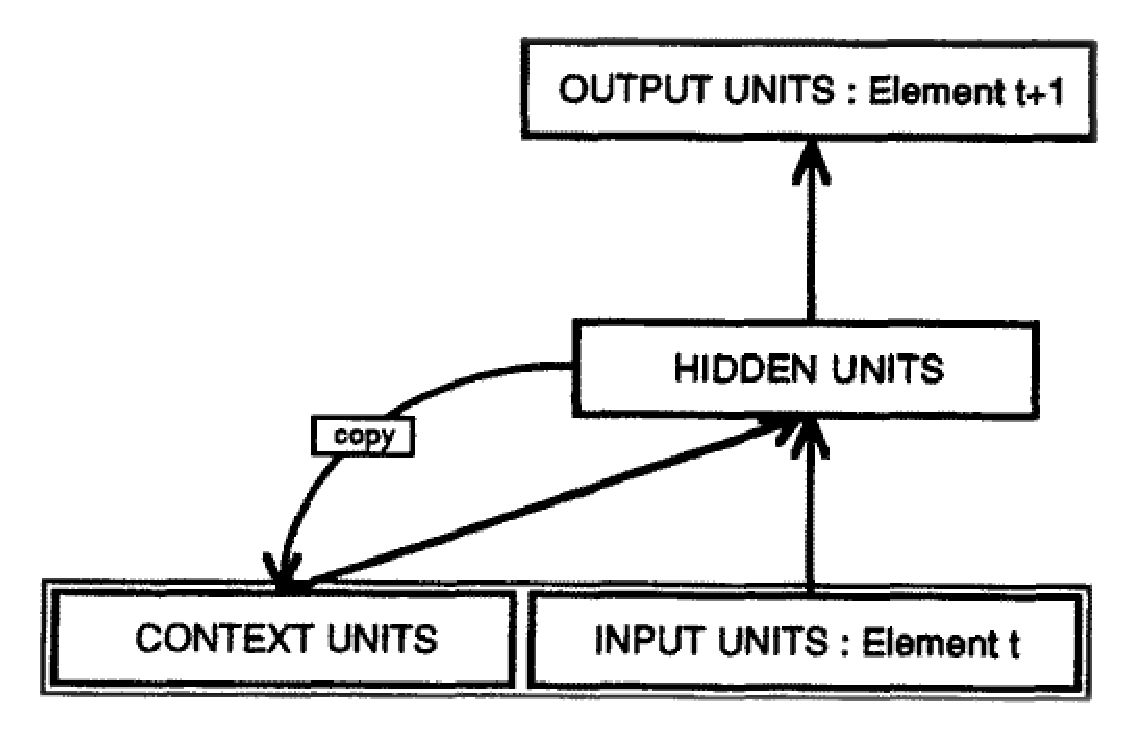
\includegraphics[width=85mm]{figures/srn.eps}
%\end{center}
%\caption{General structure of a Simple Recurrent Network (SRN) model.  Image adapted from Cleeremans and McClelland (1991).}
%\label{SRN-Model}
%\end{figure} 

\begin{figure}[t]
\begin{center}
	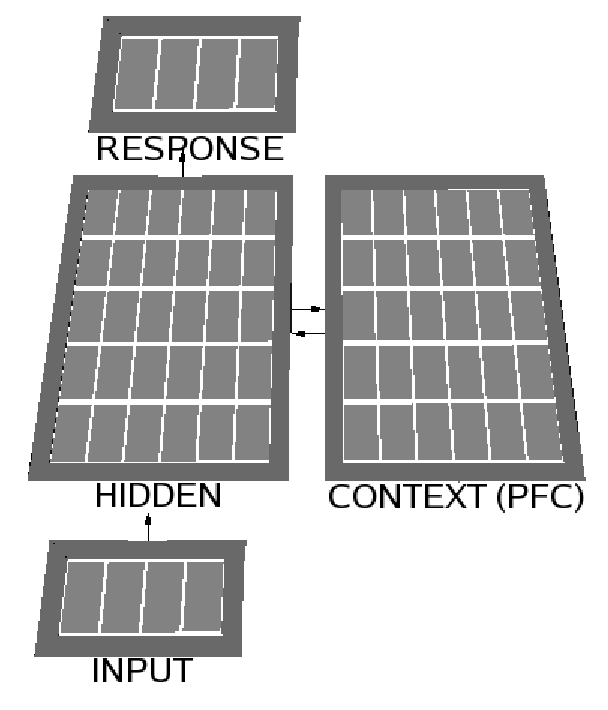
\includegraphics[width=75mm]{figures/srtt_network.eps}
\end{center}
\caption{Network Diagram of SRTT Model} 
\label{network-diagram-srtt}
\end{figure}

% Since the hidden sequential structure in the intermediate blocks of the SRTT is often complex, the information provided by the context layer is vital for the success of the model.  Importantly,
The context layer in the Cleeremans \& McClelland model played an identical functional role to the PFC in other models, actively maintaining information to modulate an input-output mapping. In this case, the context layer actively maintained information about the preceding button presses, influencing the prediction of the next button. In our executive dysfunction model, described previously, the PFC was updated in a dynamic fashion, based on learned task contingencies. In this SRTT model, the context layer is updated with each new input. Thus, the SRN context layer is analogous to the PFC in XT, with the updating ``gate'' forced to open with each new input~\cite{OReillyRC:2000:Computational}.
%~\cite{OReillyRC:2006:MWMW}.
%Since the hidden sequential structure in the intermediate blocks of the SRTT is often complex, the information provided by the context layer is vital for the success of the model.  Importantly, the context layer in this model plays an identical functional role to the PFC in other models, actively maintaining information that can be used to modulate an input-output mapping.  In our previous executive dysfunction model, the PFC actively maintained information about the currently relevant stimulus dimension (e.g., ``focus on the ink color'' in Stroop or ``sort cards based on shape'' in WCST), so as to modulate performance.  In this model, the context layer actively maintains information about the preceding button presses, allowing that information to modulate the prediction of the next button.  In our previous model, the PFC was updated in a dynamic fashion, based on learned task contingencies.  In this model, the context layer is updated with each new input presentation.  Thus, the SRN context layer is analogous to the PFC in our previous model, with the updating ``gate'' forced to open with each new input~\cite{OReillyRC:2006:MWMW}.

In order to capture the relevant sequential information, the SRN model must update the context layer in a fast and appropriate manner. This flexible updating of contextual information is precisely the cognitive mechanism we hypothesize to be suspect in people with autism. By restricting the ability of the SRN to update the context layer, mirroring the PFC updating failures that arise with weakened PFC/DA interactions in our other models, we aimed to capture the performance of people with autism. We implemented this updating restriction with a single new parameter: a probability that context layer (PFC) updating will be successful with each new input. Healthy behavior was modeled by setting this probability to one, and the probability was reduced to model ASD performance. This manipulation is analogous to reducing the efficacy of the DA-based gating signal to the PFC.  Restricting the updating of the PFC, in this manner, makes the temporally extended information stored there much less reliable, hindering the learning of complex sequential structures in the ASD model.


\subsection{Implicit Learning Simulation Results}
Model simulations were repeated $100$ times in each of the experimental conditions, with initial synaptic connection strengths randomized for each repetition. Average performance results for each block were compared to previously reported response time data for both people with autism and typically developing controls~\cite{MostofskySH:2000:Procedural}. The context layer updating probability and the response time scaling parameters that produced the lowest sum-squared deviation from the human data were identified as the best fit model.

The resulting modeled reaction times, along with previously reported human data, appear in Figure~\ref{Model-Results}. The best-fit updating probability for the autism model was found to be $0.5$. A repeated measures ANOVA on blocks 1, 2, 3, and 4 of the model results showed a significant Group by Block interaction ($p < 0.000001$). This indicates that the ASD networks demonstrated significantly less learning over the crucial training blocks (2--4) than the networks allowed to reliably update their PFC-like context layers. Thus, clear implicit learning deficits were found in the autism model.

%The simulation results match human performance both qualitatively and quantitatively, providing evidence that impairments in PFC updating can result in implicit learning deficits like those seen in people with autism.  When the healthy network is restricted to perfectly update its Context Layer (i.e., with probability one), the corresponding best-fit probability for the autism network is $0.5$, with an SSE of $652$. The corresponding scaling parameter from error to reaction time is $261.4$, the healthy base time is $458.6$ msec, and the autism base time is $534.5$ msec.  The resulting modeled reaction times, along with human data from the literature, is shown in Figure~\ref{Model-Results}.

\begin{figure}[t]
\begin{center}
%%	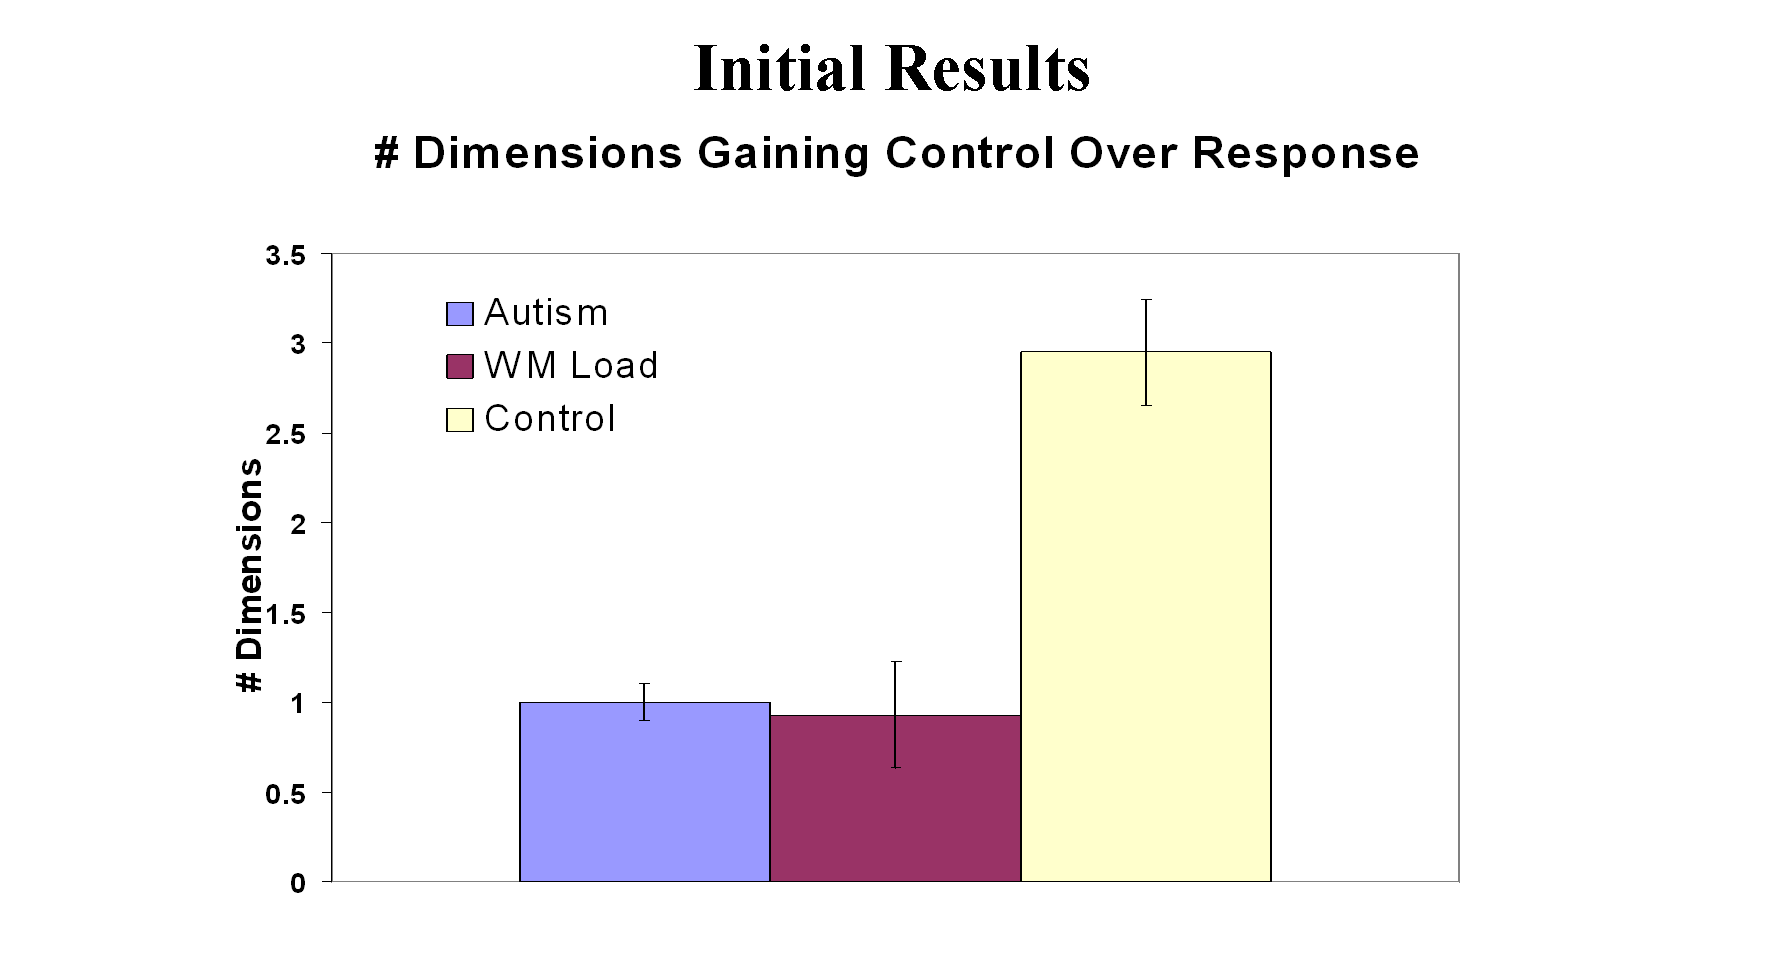
\includegraphics[width=125mm]{graphs/OS_initial_results.eps}
	\includegraphics[width=75mm]{figures/srtt_chart.ps}
\end{center}
\caption{Model Results \& Human Behavioral Data from Mostofsky
         et al. (2000)} 
\label{Model-Results}
\end{figure} 

\subsection{Summary}

Our simulation results matched human performance both qualitatively and quantitatively, providing evidence that impairments in PFC updating can result in SRTT deficits like those seen in ASD. It is interesting to note that this account posits deficits in learning temporal patterns rather than in implicit learning, per se. More information about these simulations may be found in Kriete \& Noelle~(2009).\nocite{KrieteT:2009:SRTT}

%The modeling results presented in this section suggest that, in people with autism, implicit learning deficits may be driven largely by abnormalities in DA/PFC interactions, causing inflexibility in the updating of contextual information.  Without the proper updating of actively maintained contextual information, it is essentially impossible to properly integrate temporally separated pieces of information, such as the order of items in a sequence.  Thus, our computational account highlights how PFC/DA dysfunction can lead to problems with information integration.  This is particularly interesting, since one prominent behavioral theory of autism, \emph{Weak Central Coherence}, posits that deficits in integrating contextual information lay at the core of this disorder~\cite{HappeF:1999:WCC}.  
